\documentclass[11pt]{beamer}
\usetheme{metropolis}

\usepackage[french]{babel}
\usepackage[utf8]{inputenc}
\usepackage[T1]{fontenc}
\usepackage{booktabs}
\usepackage{array}
\usepackage{graphicx}

\title{Construction d'un arbre hiérarchique hybride}
\subtitle{État d'avancement méthodologique --- résultats en cours de validation}
\date{}
\author{}

\begin{document}

\maketitle

\begin{frame}{Sommaire}
  \tableofcontents
\end{frame}

% ============================================================
\section{Point de départ}
% ============================================================

\begin{frame}{Le pipeline général}
  Maquette $\rightarrow$ Détection $\rightarrow$ \textbf{Arbre} $\rightarrow$ Code

  \vspace{1em}
  La qualité du code final dépend presque entièrement de la qualité de l'arbre
  intermédiaire --- c'est l'étape la plus fragile, celle que nous attaquons.

  \vspace{1em}
  \alert{Chaque décision qui suit répond à une question précédente --- suivons le
  fil.}
\end{frame}

% ============================================================
\section{Question 1 --- Quelle famille de méthode ?}
% ============================================================

\begin{frame}{Le paysage des méthodes UI-to-code}
  \small
  \begin{itemize}
    \item Systèmes à base de règles (REMAUI)
    \item Deep learning bout-en-bout (Pix2Code, Sketch2Code)
    \item Apprentissage par renforcement (Soselia et al.)
    \item Prompting direct de gros VLM (Design2Code)
    \item Hybride vision + deep learning (Bo et al.)
  \end{itemize}

  \vspace{0.5em}
\end{frame}

\begin{frame}{Pourquoi un hybride vision par ordinateur classique + MLLM}
  \small
  \begin{itemize}
    \item \textbf{vs règles} : nous partons d'une image brute, sans métadonnée
    \item \textbf{vs deep learning bout-en-bout} : notre arbre reste explicite et
      inspectable à chaque étape
    \item \textbf{vs prompting direct de VLM} : notre géométrie est garantie par
      calcul, jamais par prédiction
    \item \textbf{vs hybrides existants} (DCGen, ScreenCoder, VSA) : chez eux,
      Le transformeur/MLLM de VSA, le MLLM de ScreenCoder intervient encore dans la structuration elle-même
  \end{itemize}

  \vspace{1em}
  \alert{$\rightarrow$ Reste à trancher : dans quel ordre combiner calcul et MLLM ?}
\end{frame}

% ============================================================
\section{Question 2 --- Dans quel ordre ?}
% ============================================================

\begin{frame}{Deux ordres possibles, deux exemples vérifiés}
  \textbf{DesignCoder} (arXiv:2506.13663) --- le MLLM groupe en premier :
  \begin{quote}
    \small \textit{« Group the UI elements [...] into UI components. Output a
    complete hierarchical tree. »}
  \end{quote}

  \textbf{ScreenCoder} (arXiv:2507.22827) --- le MLLM positionne directement :
  \begin{quote}
    \small \textit{« queried with prompts such as `Where is the sidebar?' [...]
    returns [...] bounding boxes »}
  \end{quote}
\end{frame}

\begin{frame}{Notre choix : l'inverse, assumé}
  \begin{columns}
    \column{0.5\textwidth}
    \textbf{Étape 1}\\
    via la vision par ordinateur classique\\
    construit l'arbre complet
    \column{0.5\textwidth}
    \textbf{Étape 2}\\
    Le MLLM étiquette\\
    les nœuds déjà construits
  \end{columns}

  \vspace{1em}
  \alert{Le MLLM ne modifie jamais une position --- il attache seulement un nom.}

  \vspace{1em}
  \small L'utilisation des outils de vision par ordinateur classique garantit une structure fiable et déterministe ; les erreurs de
  raisonnement du MLLM ne peuvent plus contaminer la géométrie.

  \vspace{1em}
  \alert{$\rightarrow$ Reste à définir : que doit contenir un nœud de cet arbre ?}
\end{frame}

\begin{frame}{Image d'une maquette avant la detection via la vision par ordinateur classique}
  \centering
  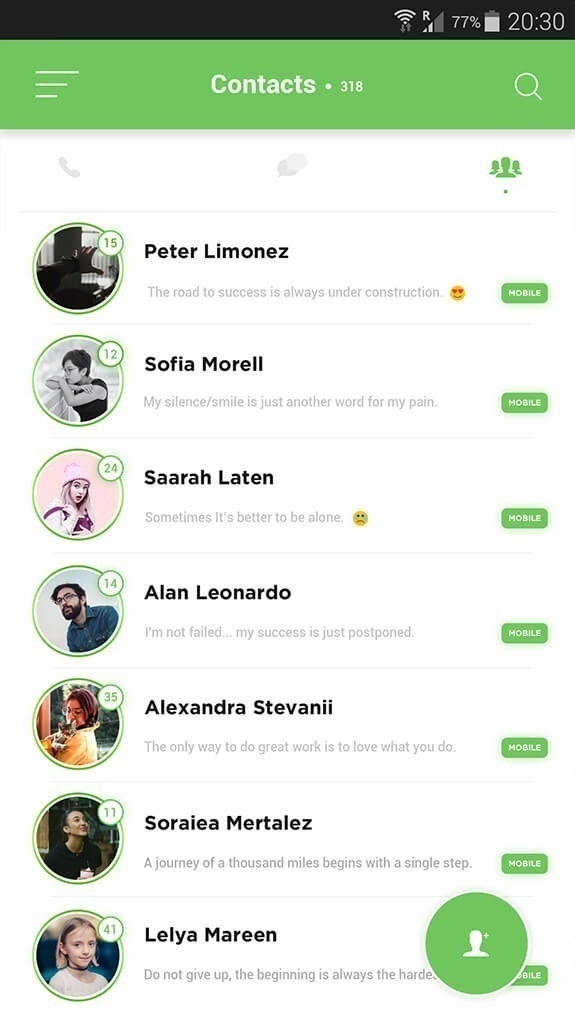
\includegraphics[width=0.4\textwidth]{images/2.jpg}
\end{frame}

\begin{frame}{Image d'une maquette apres la detection via la vision par ordinateur classique}
  \centering
  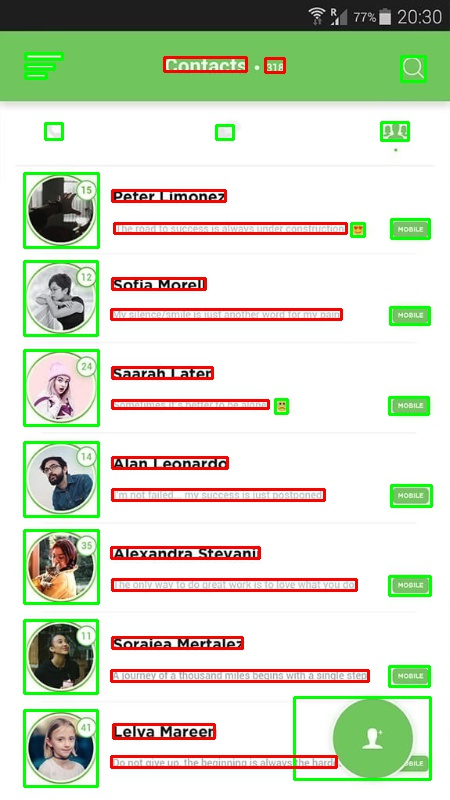
\includegraphics[width=0.4\textwidth]{images/2_uuied.jpg}
\end{frame}

% ============================================================
\section{Question 3 --- Que contient un nœud ?}
% ============================================================

\begin{frame}{Huit champs, quatre origines}
  \small
  \begin{table}
    \centering
    \begin{tabular}{lll}
      \toprule
      Champ & Origine & Source qui justifie \\
      \midrule
      id & Neutre & Zhang-Shasha (1989) --- Tree Edit Distance \\
      bbox & Détecteur & Universel (UIED, Screen Parsing) \\
      type grossier & Détecteur & Consommé par Gestalt (clustering) \\
      parent & Géométrie & Remontée et fusion \\
      children (ordonné) & Géométrie & Zhang-Shasha --- ordre significatif \\
      type géométrique & Géométrie & Prototype2Code, ReverseORC \\
      label sémantique & MLLM & Contribution centrale \\
      \textbf{hash} & Géométrie & VSA (2025) --- motif discovery \\
      \bottomrule
    \end{tabular}
  \end{table}
\end{frame}

% ============================================================
\section{Question 4 --- Sommes-nous vraiment nouveaux ?}
% ============================================================

\begin{frame}{Un vide de recherche à nuancer honnêtement}
  \textbf{VSA} (arXiv:2512.20034, déc. 2025) sépare déjà : structure $\rightarrow$
  motifs $\rightarrow$ code.

  \vspace{1em}
  \alert{Mais leur étape de structure utilise \textit{« a spatial-aware
  transformer »} --- un réseau de neurones.}

  \vspace{1em}
  
  \vspace{1em}
  \alert{$\rightarrow$ Sur quel terrain  et avec quel outil concret allons-nous
  appliquer tout cela ?}
\end{frame}

% ============================================================
\section{Question 5 --- Quel terrain et quel outil ?}
% ============================================================

\begin{frame}{Le choix du détecteur}
  \small
  \textbf{Screen Parsing} (Wu et al., UIST 2021) --- écarté :
  \textit{« trained [...] on two mobile UI datasets: AMP [...] and RICO »}

  \vspace{0.5em}
  \textbf{ImageCLEF DrawnUI 2021} --- écarté : entraîné sur du web, mais aucun
  poids ni code public trouvé.

  \vspace{0.5em}
  \textbf{UIED} (Xie et al., ESEC/FSE 2020) --- retenu : détection purement
  algorithmique, position + type grossier, sans réseau de neurones pour le sens.
\end{frame}

\begin{frame}{Pourquoi Gestalt seul ne suffit pas sur le web}
  Gestalt (Xie et al., 2022, arXiv:2206.10352) regroupe les éléments en blocs
  naturels, sans besoin d'espace vide.

  \vspace{1em}
  Évalué sur 1091 captures Android (Rico) + 20 prototypes Figma --- et
  \textbf{limité à 2-3 niveaux de profondeur}.

  \vspace{1em}
  Suffisant pour du mobile, généralement plus plat. Mais nos maquettes web
  présentent une profondeur DOM \textbf{moyenne de 17 niveaux} (min 2, max 40 ---
  DCGen, Table 1, 348 pages).

  \vspace{1em}
  \alert{Nous complétons donc Gestalt avec XY-Cut, appliqué récursivement à
  l'intérieur de chaque groupe, pour atteindre la vraie profondeur.}
\end{frame}

\begin{frame}{La chaîne complète}
  \centering
  Détecteur (UIED) \\
  $\downarrow$ \textit{position + type grossier} \\[0.3em]
  Gestalt \\
  $\downarrow$ \textit{regroupe en 2-3 niveaux (parent/children partiels)} \\[0.3em]
  XY-Cut (récursif) \\
  $\downarrow$ \textit{creuse jusqu'à la vraie profondeur} \\[0.3em]
  MLLM \\
  $\downarrow$ \textit{remplit label sémantique}\\[0.3em]
  \textbf{Arbre complet, annoté}
\end{frame}

% ============================================================
\section{État d'avancement --- à l'essai}
% ============================================================

\begin{frame}{\alert{Important} : nous testons encore, aucun résultat validé}
  \begin{itemize}
    \item Installation testée : Google Colab, puis local (WSL) suite à un
      blocage Windows sur les bibliothèques compilées
    \item Deux incompatibilités de code corrigées (bibliothèques ayant évolué
      depuis 2022)
    \item Détection brute validée sur une maquette mobile de test
    \item Biais identifié sur une capture web : navigateur et barre des tâches
      inclus par erreur --- à corriger
  \end{itemize}

  \vspace{1em}
  \alert{XY-Cut reste à écrire ; aucune mesure quantitative (Tree Edit Distance,
  TreeBLEU) n'a encore été réalisée.}
\end{frame}

\begin{frame}{Prochaines étapes}
  \begin{enumerate}
    \item Refaire les tests sur de vraies captures de pages web complètes
    \item Confirmer l'effet de \texttt{recognize\_layout()} sur la fragmentation
      du texte
    \item Écrire l'algorithme XY-Cut nous-mêmes
    \item Mesurer quantitativement une fois le pipeline complet fonctionnel
  \end{enumerate}
\end{frame}

\begin{frame}[standout]
  Merci --- questions et retours bienvenus
\end{frame}

\end{document}
